\section{Применение BERT к медицинским данным}
\subsection{Формализация задачи и обзор данных}
\subsubsection{Датасет NBME}
NBME \cite{NBME} выбран в качестве датасета для проверки алгоритма и последующей интрепретации. Задача связана с формализацией диагноза из опроса и осмотра пациента. 
В качестве данных представлены заметки о пациентах - отрывки наблюдений о каждом и признаки для каждого клинического случая, эти данные разделены на две таблицы.
\newline
Понятия о данных этого датасета:
\begin{itemize}
\item Клинический случай (clinical case): сценарий (например, симптомы, жалобы, опасения), который пациент представляет.
\item Примечание пациента (patient notes): Текст, содержащий подробную важную информацию, сообщенную пациентом во время встречи (физического осмотра и собеседования).
\item Признак (feature): Клинически значимая концепция. В рубрике описаны ключевые понятия, относящиеся к каждому конкретному случаю.
\end{itemize}
Обучающая и тестовые выборки разбивают данные по клиническому случаю, примечанию пациента и признаку (либо признакам), задача заключается в указании части примечания, содержащей информацию о признаке. 
\subsubsection{Постановка и метрика качества}
Ответы представлены парами индексов \textit{\{ i, k \}}, возможно несколько для 1 сэмпла. Как раз такие пары и должна научиться строить модель.
Задача не очевидна, но ее можно свести к классификации посредствам перехода к следующему восприятию ответов:
позитивным сэмплом (речь о сабсэмпле-индексе для реального сэмпла) называть входящие в обозначеный отервал индексы; по факту от модели требуется бинарно классифицировать все индексы, вместо пары \textit{\{ i, k \}} максимизируя вероятности для $\forall k \in [i,j)$ для верных.
\newline
Предложенная метрика для данных в соответствующем данным соревнованию - специально заданная \textit{f1score}. Обычный вид метрики:
\begin{gather*}
    \textit{TP - верно предсказанный позитивный сэмпл,}\\ 
    \textit{FP - неверно предсказанный позитивный сэмпл,}\\
    \textit{FN - неверно предсказанный негативный сэмпл}\\
    \nonumber Recall = \frac{TP}{TP+FN}\\
    \nonumber Precision = \frac{TP}{TP+FP}\\
    f1score = 2*\frac{Recall*Precision}{Recall+Precision}
\end{gather*}
Метрика для этой задачи имеет такую же формулу, но отличается более подходящим определением \textit{TP, FP, FN}:
\begin{gather*}
    \textit{TP - индекс входит в пересечение предсказания и лейбла,}\\
    \textit{FP - входит в предсказанный, но не в лейбл,}\\
    \textit{FN - входит в лейбл, но не в предсказанный отервал}
\end{gather*}
Важное свойство метрики заключается в том, что она как среднегармоническое мягко приближает минимум метрик \textit{Полноты} и \textit{Точности}, достаточно справедливо оценивая качество модели в терминах ошибки первого и второго рода, что вытекает из стандартного определения и сохраняется в описанном для этой задачи. 
\newline
После выбора всех значащих индексов их нужно превести в вид \textit{\{ i, k \}} и разделить ";" для соответсвия требованиям при помощи несложного процесса парсинга.
% \subsubsection{Explanatory Data Analysis}
% Полезно может быть дополнительно исследовать данные, в ходе EDA можно получить какие-то важные характеристики.
\subsection{Решение задачи}
Для решения задачи использовался претренированая модель BERT Base Uncased и соответствующий токенайзер (работа проведена с использованием фреймверков \textit{pytorch} и \textit{hugging face transformers}). Поверх нее были добавлены 3 линейных слоя с дропаутом - оператором, случайно зануляющим некоторые каналы с вероятностью \textit{p} при тренеровке и домножающим остальные значения на $\frac{1}{1-p}$. Применение техники регуляризует сети по средствам контроля коадаптации искусственных нейронов.
\newline
Применяя \textit{[CLS]} токен и линейные слои получаются 1-мерные массивы, для получения вероятности требуется применить к ним фунцию $Sigmoid(x) = \frac{1}{1+e^{-x}}$. В качестве функции потерь применялась \textit{Бинарная Кросс Энтропия}:
\begin{equation} \label{BCE}
    BCE(x,y)=\{l_{j}\}, l_{j} = −w_{n}\left(y_{n}\times log x_{n}+(1−y_{n})\times log (1 - x_{n})\right)
\end{equation}
Для оптимизации весов в процессе обученния использовался \textit{AdamW}, версия оптимизатора с адаптивными моментами и переработанным механизмом регуляризации на основе весов сети, файн-тюнинг длился 3 эпохи с постоянным размером шага обучения $lr=10^{-5}$. Также для более стабильного процесса оптимизации приенялась техника \textit{клипинга градиента} - ограничения значений градиента пороговыми значениями ($grad := max(grad, threshhold)$), обеспечивающий более плавную сходимость без \textit{взрывов градиента}.
Результат на валидационной выборке после 3 эпох файнтюнинга:
\begin{center}
\begin{tabular}{ |c|c| } 
 \hline
 Метрика & Значение\\ 
 \hline
 Accuracy & 0.99307\\ 
 \hline
 Precision & 0.725280\\ 
 \hline
  Recall & 0.85514\\ 
 \hline
  f1 & 0.78488\\ 
 \hline
\end{tabular}
\end{center}

\begin{figure}[h]
\caption{Изменение функции потерь в ходе дообучения}
\centering
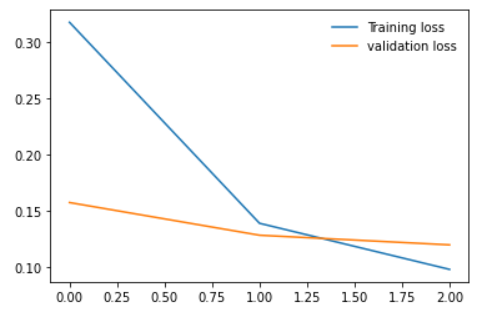
\includegraphics[width=0.5\textwidth]{loss_bert.png}
\label{loss}
\end{figure}

\subsection{Интерпретация алгоритма}
\subsubsection{Значение Шэпли}
Как было обозначенно в начале, алгоритмы требуется интерпретировать для последующей оценки реальными экспертами. Одним из основных методов является оценка влияния входных данных на результат. При помощи \textit{SHAP (SHapley Additive exPlanation)} можно оценить вклад входных признаков на ответ модели. Несмотря на то, что \textit{SHAP} предназначен для оценки вклада тгроков в каолиционной игре и вычисления основаны на расчете маржинального вклада игроков, при помощи интерпретации призников как игроков и вычисления маржинального вклада при помощи сэмплинга \cite{model_expl}, эти значения будут являться хорошим критерием при анализе модели машинного обучения\cite{shap_models}.
\subsubsection{Анализ модели при помощи SHAP}
Анализ BERT моделей с классификацией последовательности представленный в \cite{bert_shap} подразумевает вычисления для каждого токена входной последовательности. Для применения подхода к текущей задаче восприятие разметки как бинарной классификации каждого члена последовательности так же полезно. В данном случае вычислен \textit{SHAP} для пар элемент \textit{i} - вероятность для элемента \textit{j}.
\newline
В результате для предложения 
\begin{figure}[h]
\centering
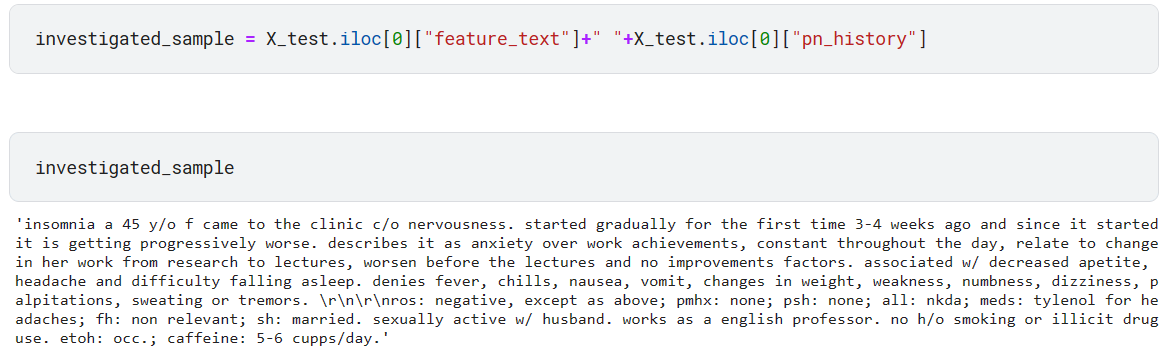
\includegraphics[width=0.75\textwidth]{sample.png}
\label{sample_txt}
\end{figure}
получилась матрица \ref{shap_mt}.

\begin{figure}[h]
\caption{Карта SHAP Values}
\centering
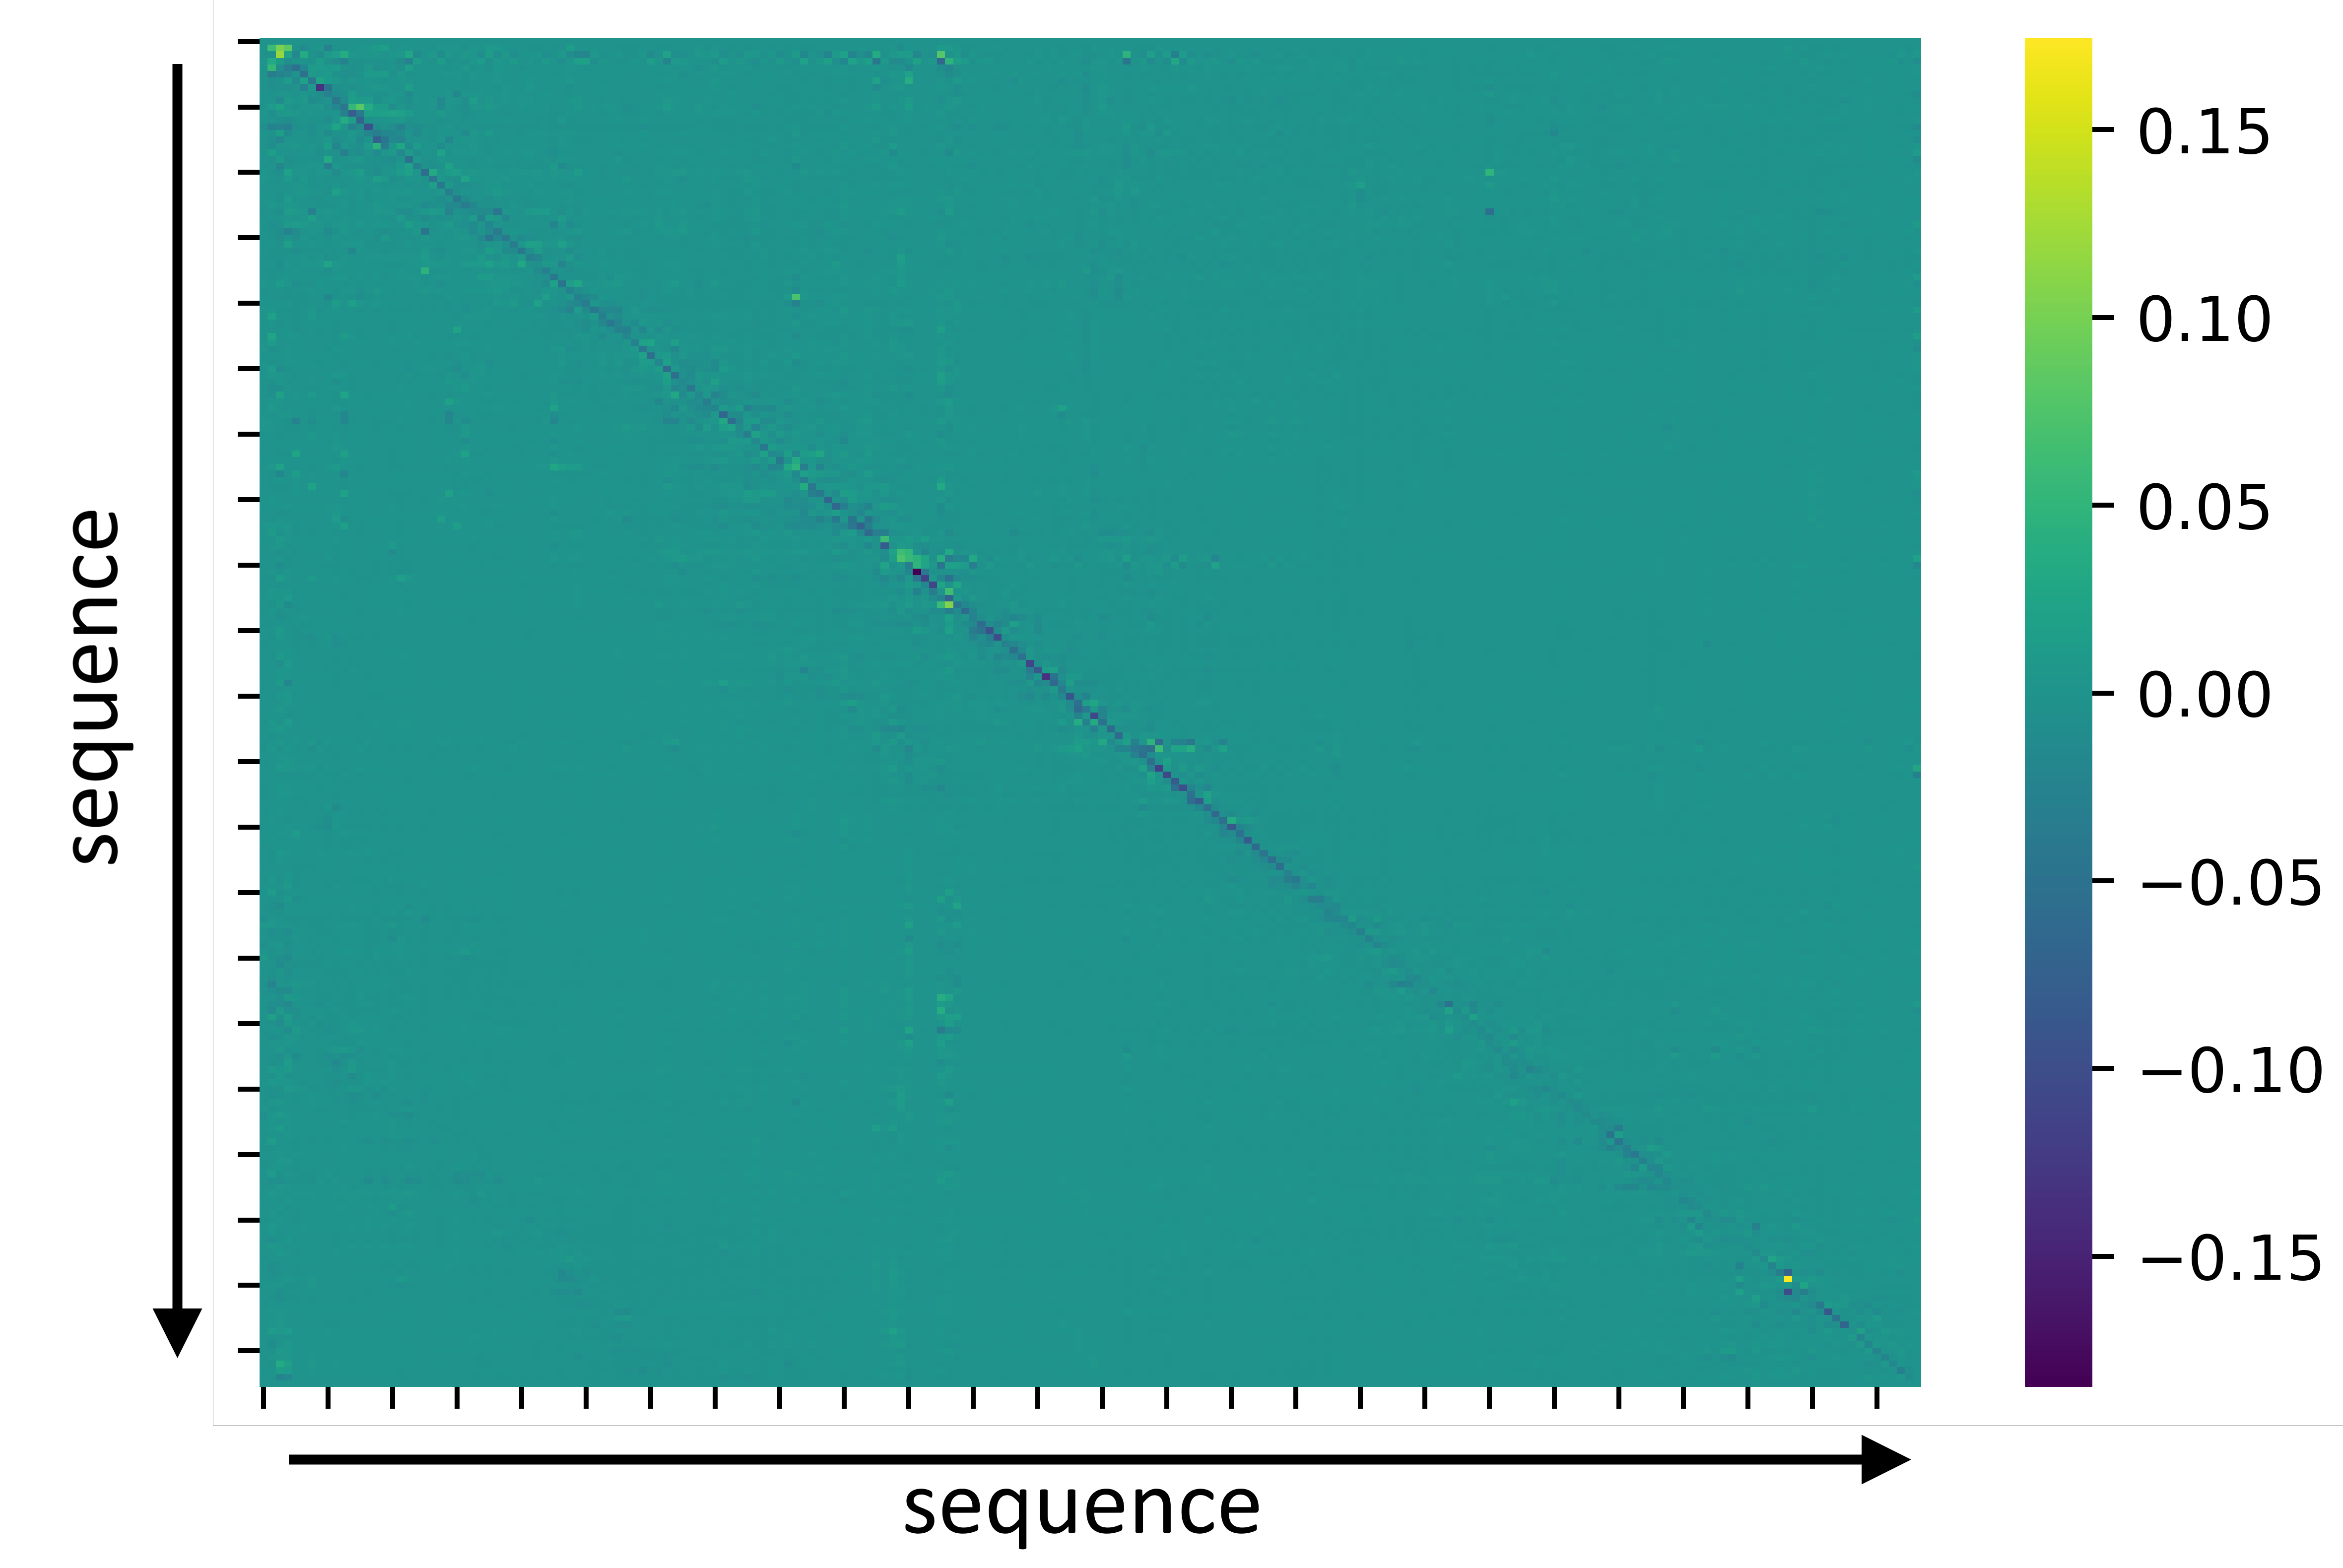
\includegraphics[width=1\textwidth]{sequence_shap_map.png}
\label{shap_mt}
\end{figure}
Пользуясь такой матрицей можно по индексу в последовательности найти слова, ответственные за принятие решения сетью и понять логику получения ответа для какого-то региона.
\begin{figure}[h]
\caption{Карта SHAP Values с выделениями: красными рамками выделены токены с повышенными положительными SHAP; \textit{a,b} и \textit{c} соответствуют 1 найденному региону, при этом элементы в \textit{b} наиболее близки к диагонали, то есть токены самого региона вложились в повышение вероятности, а \textit{a} и \textit{c} находятся ранее и после региона в последовательности, выступили в качестве контекста.}
\centering
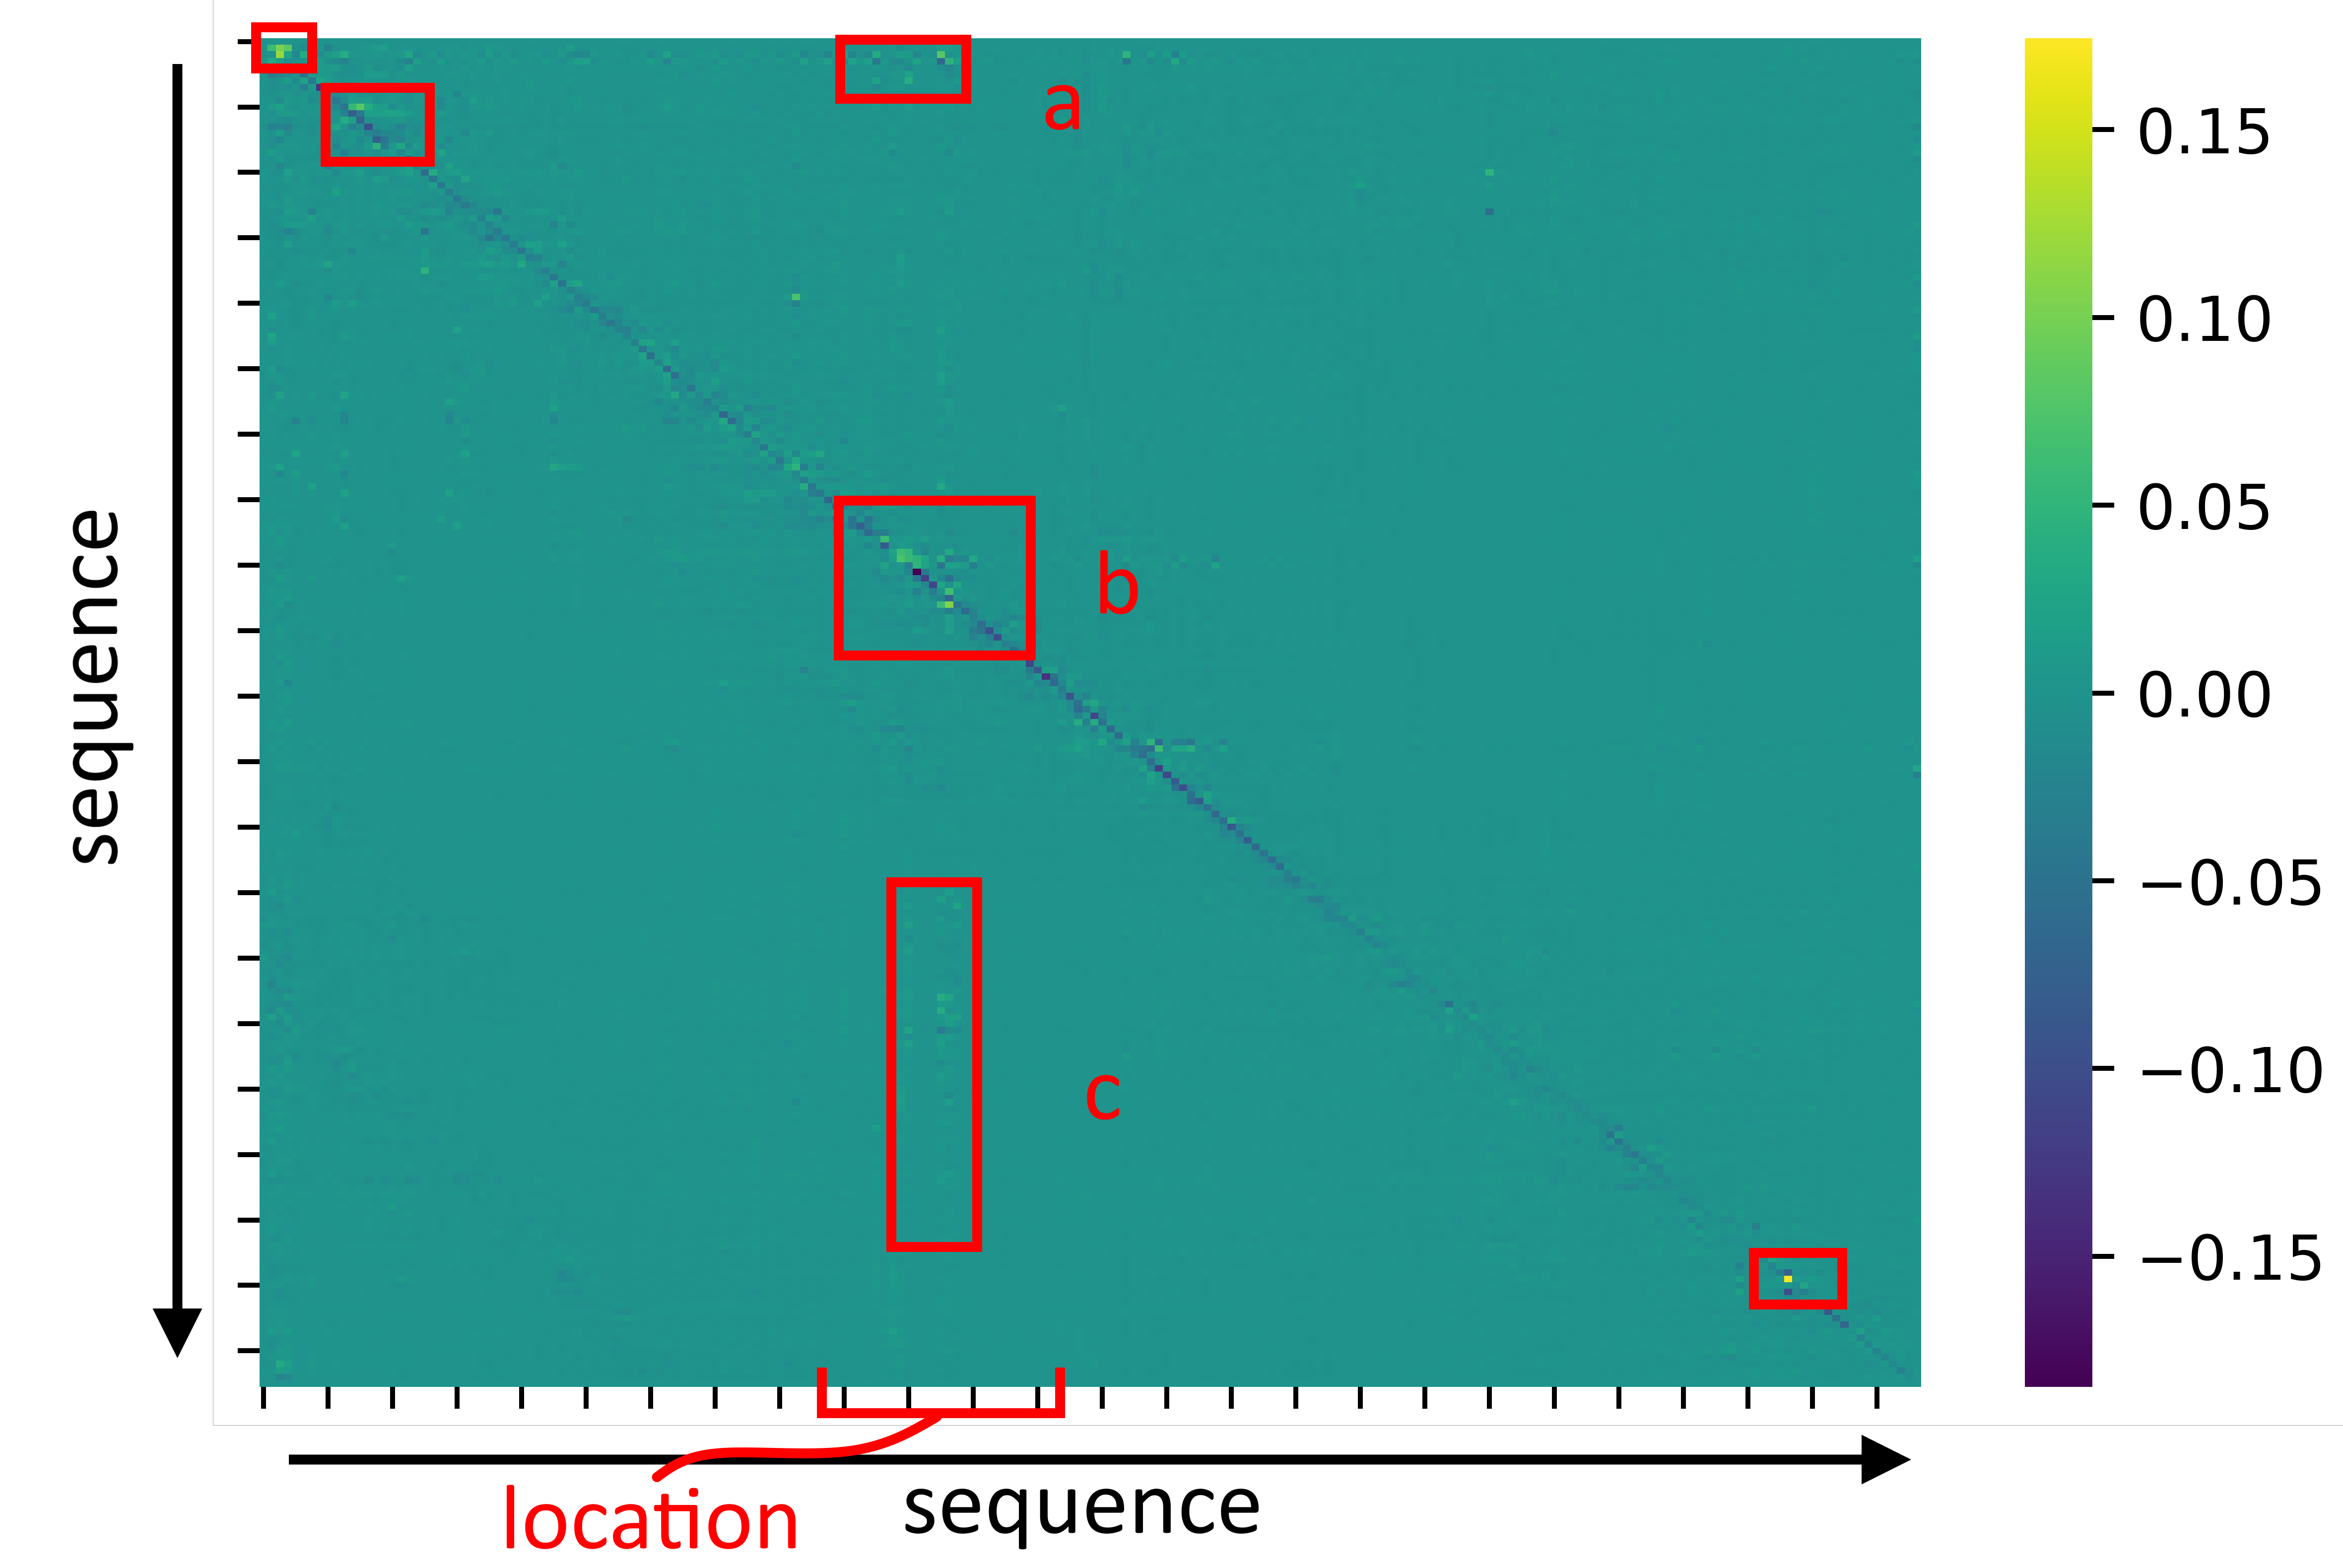
\includegraphics[width=0.75\textwidth]{sequence_shap_map_loc_annot.png}
\label{shap_mt_alloc}
\end{figure}